\documentclass[10pt]{beamer}

\mode<presentation> {

% \usetheme{Berlin}  % Squares
\usetheme{Madrid}  % Circles & dense
% \usetheme{Frankfurt}  % Cirles

\setbeamertemplate{headline}{%
\leavevmode%
  \hbox{%
    \begin{beamercolorbox}[wd=\paperwidth,ht=2.5ex,dp=1.125ex]{palette quaternary}%
    \insertsectionnavigationhorizontal{\paperwidth}{}{\hskip0pt plus1filll}
    \end{beamercolorbox}%
  }
}

\setbeamertemplate{navigation symbols}{}  % To remove the navigation symbols from the bottom of all slides uncomment this line

% \useoutertheme{miniframes}
% \useinnertheme{circles}

}

\usepackage{graphicx}
\usepackage{booktabs}
\usepackage{fontspec}
\usepackage{amsmath}
\mathchardef\mhyphen="2D % Define a "math hyphen"
\usepackage{caption}
\usepackage{xunicode}
\usepackage{xltxtra}
\usepackage{xecyr}
\usepackage{hyperref}
\usepackage{amsthm}
\usepackage{blindtext}

\usepackage{polyglossia}
\setdefaultlanguage{russian}
\setmainfont[Mapping=tex-text]{CMU Serif}
\setsansfont[Mapping=tex-text]{CMU Sans Serif}
\setmonofont[Mapping=tex-text]{CMU Serif}

\makeatletter
\DeclareUrlCommand\ULurl@@{%
  \def\UrlFont{\ttfamily\color{blue}}%
  \def\UrlLeft{\uline\bgroup}%
  \def\UrlRight{\egroup}}
\def\ULurl@#1{\hyper@linkurl{\ULurl@@{#1}}{#1}}
\DeclareRobustCommand*\ULurl{\hyper@normalise\ULurl@}
\makeatother

\newcommand\TODO[1]{\textcolor{red}{{\Large TODO: #1}}}
\newcommand\NaN{\textcolor{red}{NaN}}
\newcommand{\X}[1]{X_{\texttt{#1}}}
\newcommand{\Xaux}{\X{aux}}
\newcommand{\Xdata}{\X{data}}
\newcommand{\Xtrain}{\X{train}}
\newcommand{\Xtest}{\X{test}}
\newcommand{\Xgen}{\X{gen}}
%-------------------------------------------------------------------------------
%	TITLE PAGE
%-------------------------------------------------------------------------------
\title[Управляемая генерация текста]{Управляемая генерация текста c использованием механизма внимания%Controllable text generation with small data using auxiliary in-domain enrichment
}
\author[Беляев Станислав]{
Беляев Станислав\texorpdfstring{\\ Научный руководитель: Николенко Сергей Игоревич}{}
}
\institute[СПбАУ]
{
Санкт-Петербургский Академический Университет
}
\date{18 июня 2018}
\begin{document}
%-------------------------------------------------------------------------------
%	PRESENTATION SLIDES
%-------------------------------------------------------------------------------
\begin{frame}

% Добрый день, сегодня я презентую диплом по теме *. Мой научный руководитель *.

\titlepage
\end{frame}
%-------------------------------------------------------------------------------
\section{Введение}
\begin{frame}
\frametitle{Введение}
\framesubtitle{Задача генерации}

% Опишем постановку задачи.
% Современное глубокое обучение основано на способности вычислительных графов быть дифференцируемыми. При переходе к дискретным значениям старые подхо- ды перестают работать, поэтому приходиться строить отображения дискретного про- странства в непрерывное, что так или иначе ведет к проблемам с оптимизацией. За- дача генерации текста усложняется еще и тем, что при увеличении длины входных последовательностей быстро растет сложность по поддержанию связности, правдопо- добия и разнообразия генерируемых сэмплов.
% В данной работе, мы будем фокусировать на задаче генерации, универсальной задачи из статистики по восстановлению распределения многомерных данных. *. pmodel, в дальнейшем, используется для порождения новых примеров.
% В качестве данных мы будем рассматривать текстовых данные: *
% Существующие решения обладают рядом проблем: *

Нейронным сетям удается эффективно обобщать зависимости для данных, имеющих \textbf{непрерывное} представление в $\mathbb{R}^n$ (картинки, видео). 

В \textbf{дискретном} же пространстве операции теряют свойство дифференцируемости, что ведет к трудностям при оптимизации.

\begin{block}{Задача генерации (порождения)}
    По подвыборке $X_{\texttt{train}} \subset X$ генеральной совокупности $X$, распределенной по $p_{\texttt{data}}$, построить (явно или неявно) распределение $p_{\texttt{model}}$, приближающее реальное.
\end{block}

Возьмем в качестве $X$ текстовые данные (последовательность символов из конечного алфавита). Недостатки существующих порождающих моделей для текста:
\begin{itemize}
    \item Низкая связность или вариативность при генерации длинных примеров
    \item Невозможность эффективно использовать неразмеченные данные при генерации с условием
    \item Отсутствие интерпретируемости
\end{itemize}

\pagebreak

\end{frame}
%-------------------------------------------------------------------------------
\begin{frame}
\frametitle{Введение}
\framesubtitle{Цель}

% В общем и целом, задача генерации текста остается нерешенной, или, по крайней мере, решенной недостаточно хорошо, чтобы стать полезным инструментом для помощи человеку в реальных задачах.
% Поэтому целью: *
% Нужно решить задачи: *
% Постановка цели частично диктуется конкретными применениями в индустрии. Очень часто, входные данные обладают частично размеченными свойствами, набо- ром которых мы хотим параметризовать генерацию. Например, мы хотим написать универсальный генератор текстовых условий задачек по заданным темам для он- лайн курса по программированию, возможно облегчив работу авторам и составите- лям. Также, одно из возможных применений - генерация молекулярных структур по входному представлению SMILES [57] в виде последовательности дискретных величин (эквивалентных словам) по заданными характеристикам.

\underline{Целью} данной работы является разработка генеративной модели, позволяющей производить эффективную, управляемую и интерпретируемую генерацию текстовых данных с увеличенной длиной в условиях данных с частичной разметкой, поддерживая \textit{связность}, \textit{правдоподобие} и \textit{разнообразие} генерируемых примеров. Решение будет основываться на применении идей механизма \textbf{внимания} (attention) из глубокого обучения.

\underline{Задачи}:
\begin{itemize}
    \item Проанализировать предметную область и существующие модели.
    \item Выбрать и предобработать данные для обучения и тестирования.
    \item Выбрать метрики для оценки результата.
    \item Придумать и реализовать способы, позволяющие эффективно справляться существующими проблемами.
    \item Произвести сравнение подходов и анализ результатов.
\end{itemize}


\end{frame}
%-------------------------------------------------------------------------------
\section{Данные}
\begin{frame}
\frametitle{Данные}
\framesubtitle{Описание}

% Опишем данные, которые мы будем использовать для тестирования.
% *
% Зачем использовать данные с частичной разметкой? Дело в том, что найти текст без разметки легко, а с разметкой сложно. Нам не нужно вручную искать зависимости, нейросеть сама сумеет все обобщить, нужно только подсказать ей разметку.
% *, подробно про 30
% Мы не делаем никаких строгих предположений о структуре данных, кроме после- довательности из дискретных значений. Таким образом, в дальнейшей работе постро- енная модель может быть использована для генеративных задачах в другой области.

Каждый $x \in X$ - цельный законченный отрывок длиной в пару предложений c частично размеченным свойством. 

Для размеченной части мы возьмем Стэнфордский датасет (\textbf{SST}), основанный на базе данных отзывов о фильмах. Неразмеченная часть взята из той же области, но из другого набора данных (\textbf{IMDB}).

\newcommand{\bos}{\langle bos \rangle}
\newcommand{\eos}{\langle eos \rangle}
\newcommand{\unk}{\langle unk \rangle}
\newcommand{\pad}{\langle pad \rangle}

\begin{itemize}
    \item Разметка - бинарное категориальное свойство эмоциональной окраски
    \item Ограничение на длину предложения - $30$ слов
    \item $30000$ сэмплов для обучения, по $3000$ для валидации и тестирования
    \item BPE encoding для токенизации, позволяет абстрагироваться от языка.
    \item Ограничение на размер словаря - $15000$
    \item $4$ служебных слова - $\bos$, $\eos$, $\unk$ и $\pad$ - символы начала, конца, пустоты и отступа. Используются для обрамления начала/конца и объединения примеров в батч для обучения.
\end{itemize}

\end{frame}
%-------------------------------------------------------------------------------
\section{Метрики}
\begin{frame}
\frametitle{Метрики}
\framesubtitle{Описание}

% Мы берем и тренируем модель, дальше можем посчитать метрики на xtext и xgen
% *
% Упомянуть о преимуществах bleu над Perplexity (работа с сырым текстом, не делаем предположений о модели)
% Помимо этого можно прибегнуть с помощи ассессоров и специальных сервисов для оценки (Толока, MTURK)

Автоматические метрики для $W \in \Xtest$ и новых сэмлов $W \in \Xgen$
\begin{block}{Perplexity (связность, правдоподобие)}
    $PP(W) = P(w_1w_2w_3\dots w_{|W|})^{-\frac{1}{|W|}} = \left[\prod\limits_{i=1}^{|W|}{\frac{1}{P(w_i|w_1\dots w_{i-1})}}\right]^{\frac{1}{|W|}}$
\end{block}
\begin{block}{BLEU (правдоподобие)}
    $BLEU(W_1, W_2) \in [0, 1], ~ \texttt{N-gram'ая схожесть, усредненная по примерам}$
\end{block}
\begin{block}{Self-BLEU (разнообразие)}
    $Self \mhyphen BLEU(S) = \frac{1}{|S|} \sum\limits^{|S|}_{i=1}{BLEU(\{S_i\}, S \setminus \{S_i\})}$
\end{block}

\end{frame}
%-------------------------------------------------------------------------------
\section{Генерация}
\begin{frame}
\frametitle{Генерация}
\framesubtitle{Таксономия генеративных моделей}

% Следуя, можно составить Таксономию ген моделей в зависимости от ...

\begin{figure}[H]
\centering
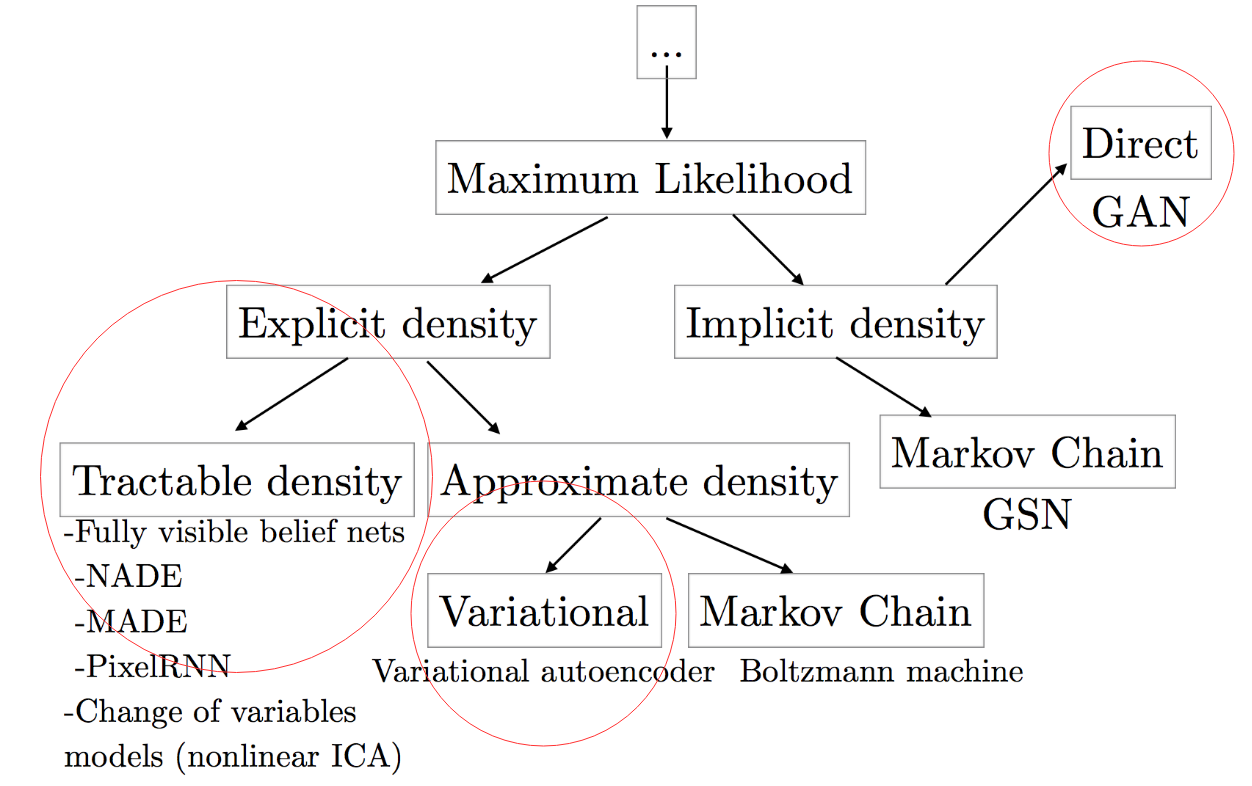
\includegraphics[width=0.85\textwidth]{images/gen_taxonomy2.png}
\caption*{Ian Goodfellow "NIPS 2016 Tutorial: Generative Adversarial Networks", 2017}
\end{figure}

\end{frame}
%-------------------------------------------------------------------------------
\begin{frame}
\frametitle{Генерация}
\framesubtitle{Рекуррентные нейронные сети (RNN)}

% явно моделируют вероятность, оптимизируют с кросс энтропией "реального"
% К достоинствам можно отнести:
% • Эффективное и простое обучение: одна ошибка, один градиент, целый набор приемов по оптимизации.
% • Расширяемая и простая реализация. RNN - базовая модель, поэтому она часть берется за основу и расширяется в сторону увеличения скорости тренировки, предотвращения переобучения, повышения интерпретируемости и глубины. К известным методам [6] можно отнести: multi-layer rnn, bidirectional rnn [44], dropout [55], scheduled sampling [43], attention [35], ensembling [56], hierachy [8], sru [29] и некоторые другие.
% • Эффективное сэмплирование. Стоимость получения сэмпла низкая, возможно оценить совместную вероятность для подсчета метрик (Формула 7), а также расширить алгоритм генерации эвристиками и регуляризацией.
% К недостаткам относятся:
% • Небольшая эффективность по метрикам и быстрая потеря связности начала с концом. Bengio [6], к примеру, связывает это с отсутствием изначального пред- ставления генерируемого сэмпла. Мы начинаем генерацию из пустоты, на ходу, слово за словом пытаясь создавать правдоподобный экземпляр, что приводит к плохой связности (coherence) при генерации.
% • RNN работает только в условиях полной разметки данных. Если же данные размечены плохо или на части данных отсутствует разметка вовсе, то учесть это в стандартной рекуррентной нейронной сети - нетривиальная задача.
% • Управляемаягенерация.ЧтобызадатьначальныеусловиядлягенерациивRNN, можно конкатенировать параметры условия с входом xi на каждом шаге генера- ции (out-of-band) или добавить свойства текста в сам текст в качестве префикса и суффикса, тогда можно начинать генерацию с нужного префикса (in-band). Оба эти подхода работают плохо даже на самых простых данных [64].
% В общем и целом, RNN - хорошая базовая модель, недостатки которой пытаются преодолеть в других подходах.

\begin{columns}
    \begin{column}{0.7\textwidth}
        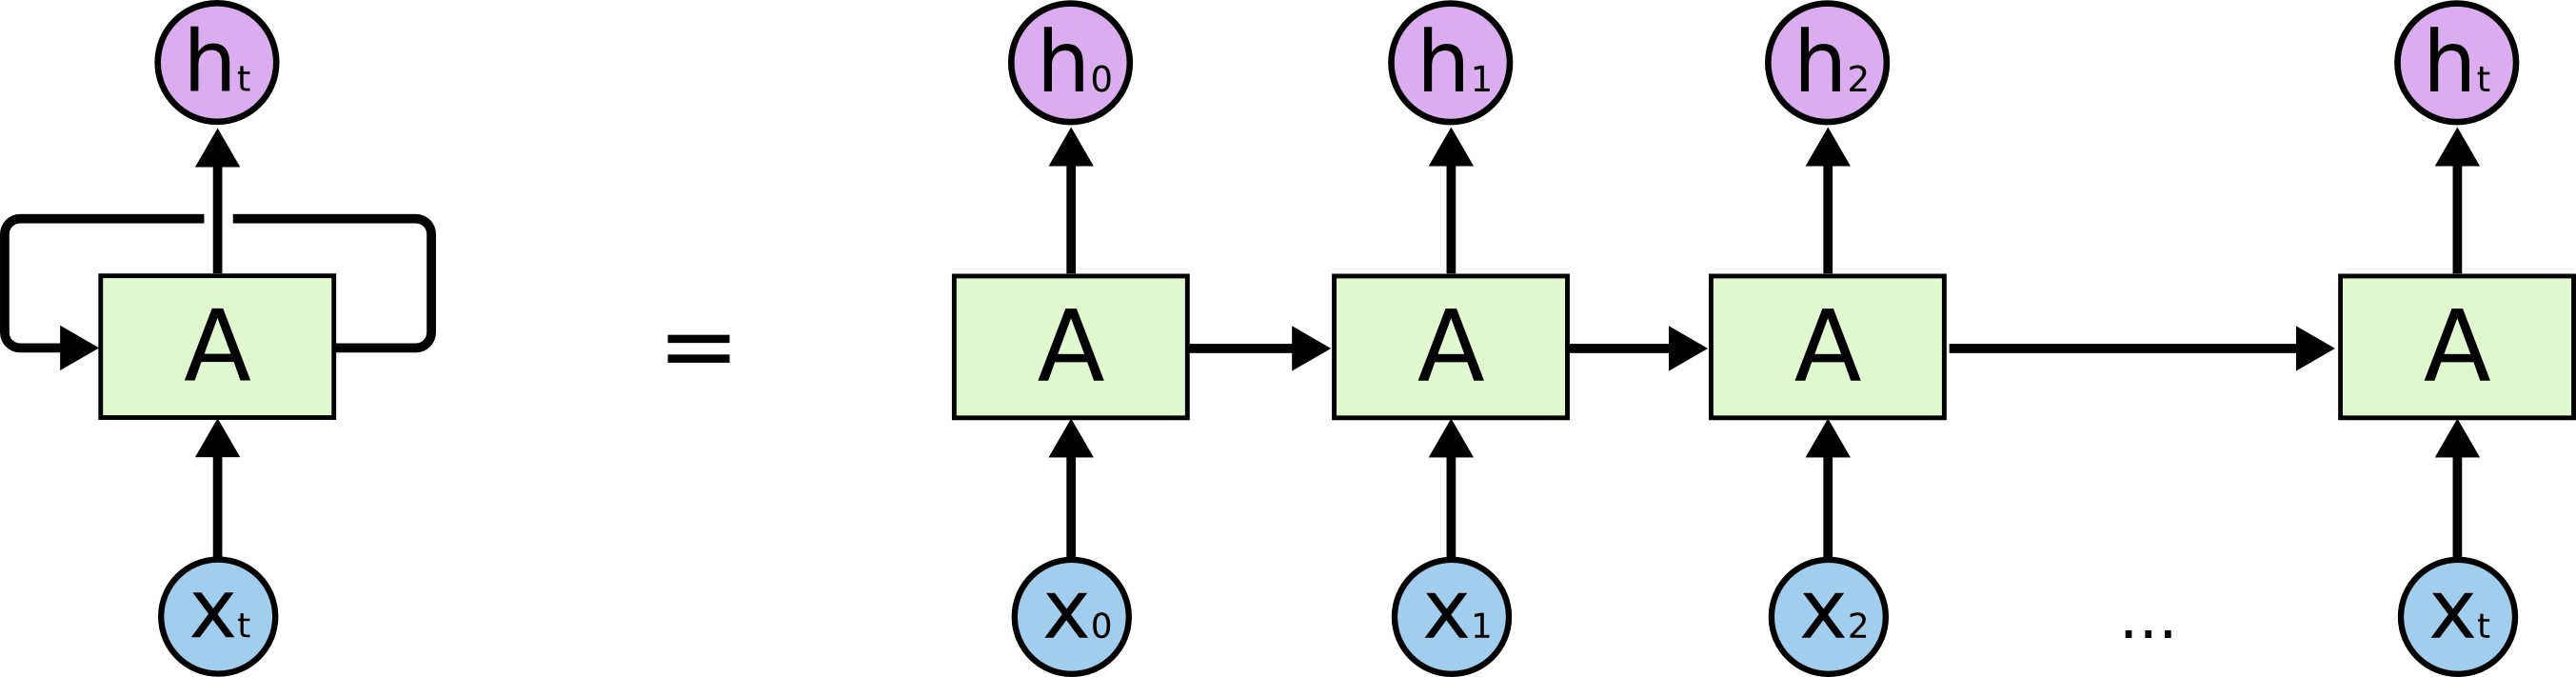
\includegraphics[height=0.25\textheight]{images/rnn_unrolled.png}
    \end{column}
    \begin{column}{0.3\textwidth}
        $p(x) = \prod\limits^{|x| - 1}_{i=0}{p(x_i | x_{<i})}$
    \end{column}
\end{columns}

Преимущества:
\begin{itemize}
    \item Эффективное и простое обучение
    \item Расширяемая и простая реализация
    \item Эффективное сэмплирование и оценивание совместной вероятности
\end{itemize}

Недостатки (Bengio, 2017):
\begin{itemize}
    \item Небольшое правдоподобие и связность
    \item Работает только в условиях полной разметки данных
    \item Неудачные механизмы управляемой генерации
    \begin{itemize}
        \item Расширение данных (in-band)
        \item Расширение архитектуры (out-of-band)
    \end{itemize}
\end{itemize}

\end{frame}
%-------------------------------------------------------------------------------
\begin{frame}
\frametitle{Генерация}
\framesubtitle{Генеративные состязательные сети (GAN)}

% рассказать про ганы
% проблема mode collapsing

\begin{columns}
    \begin{column}{0.35\textwidth}
        \begin{center}
            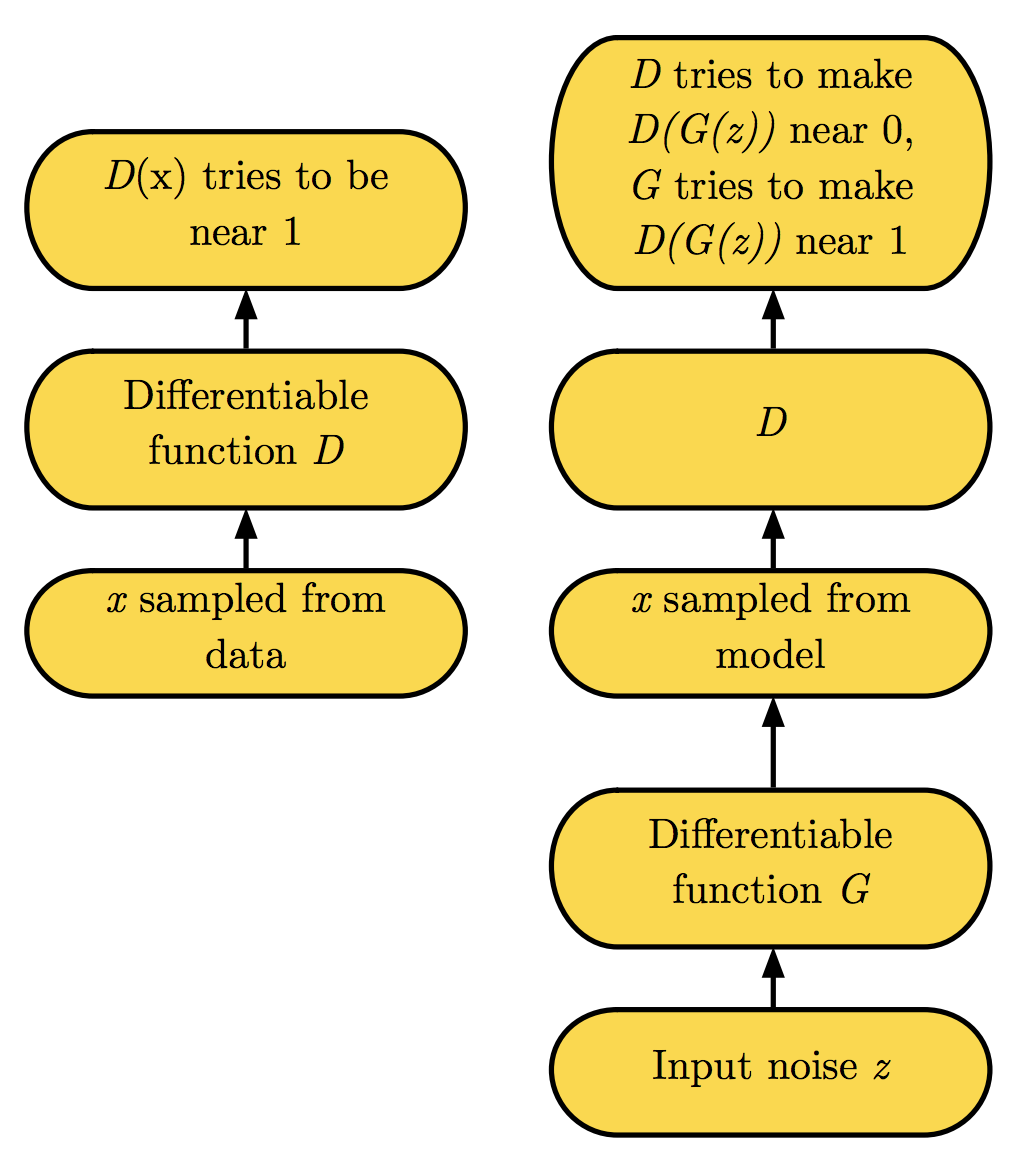
\includegraphics[width=\textwidth]{images/gan_fw.png}
        \end{center}
    \end{column}
    \begin{column}{0.65\textwidth}
        \begin{center}
            \vskip-8mm
            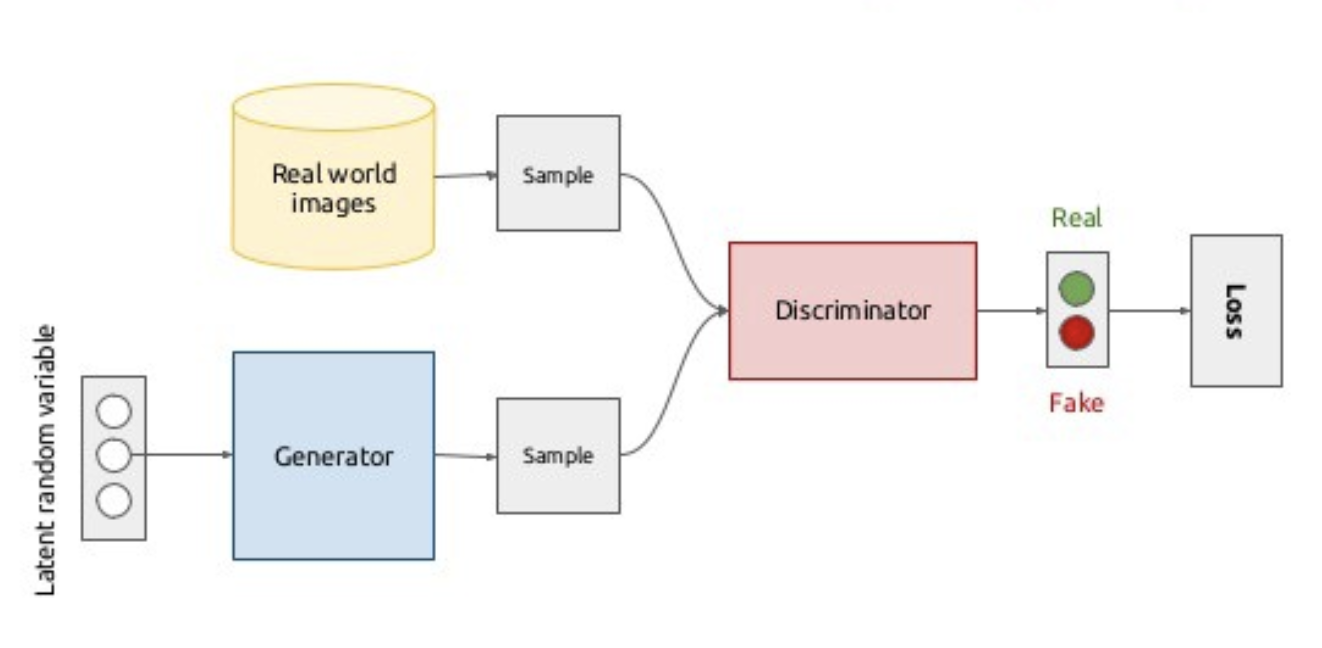
\includegraphics[width=\textwidth]{images/fan_ov.png}\\
            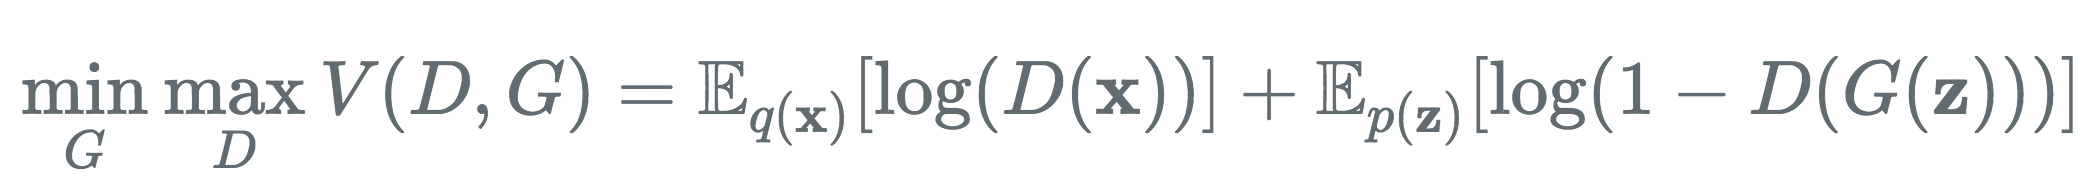
\includegraphics[width=\textwidth]{images/gan_loss.png}\\
            \vskip2mm
            Для дискретных значений (Goodfellow, 2017):
            \begin{itemize}
                \item REINFORCE (SeqGAN, LeakGAN)
                \item GumbelSoftmax (GSGAN)
                \item Embeddings ($\mathbb{N} \Rightarrow \mathbb{R}^n$)
            \end{itemize}
        \end{center}
    \end{column}
\end{columns}

\end{frame}
%-------------------------------------------------------------------------------
\begin{frame}
\frametitle{Генерация}
\framesubtitle{Вариационный автоэнкодер (VAE)}

% Ошибка - сумма ошибки восстановления и kl-терм, имеющий интерпретацию в виде регуляризации на форму латентного пространства.

\begin{center}
    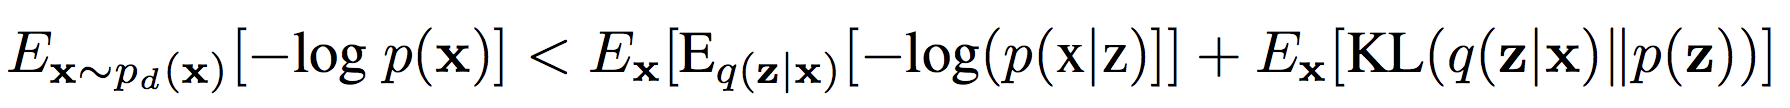
\includegraphics[width=0.8\textwidth]{images/elbo.png} \\
    \vskip-5mm \\
    \begin{columns}
        \begin{column}{0.5\textwidth}
            VAE - вариационное продолжение автоэнкодера для генерации.
            
            Чтобы правильно обучить VAE для текста (Bowman et al., 2014), нужно:
            \begin{itemize}
                \item Постепенно плавно увеличивать вес ошибки kl-терма.
                \item Реализовать дропаут для декодера, чтобы тот не обучался быстрее энкодера.
            \end{itemize}
        \end{column}
        \begin{column}{0.5\textwidth}
            \begin{center}
                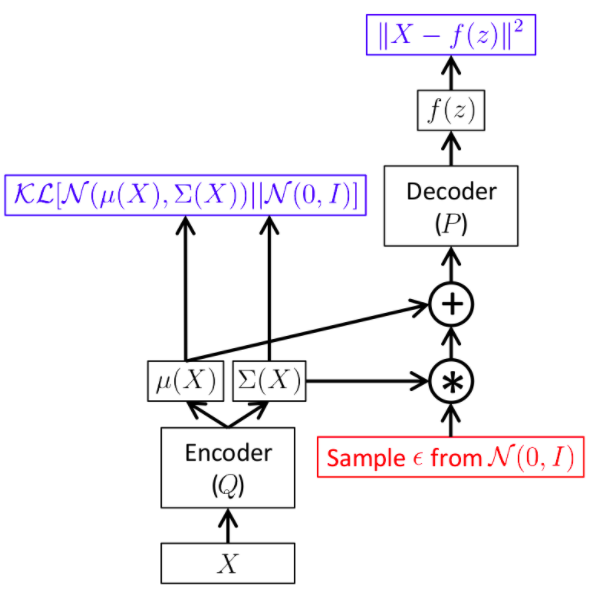
\includegraphics[width=\textwidth]{images/vae_terms.png}
            \end{center}
        \end{column}
    \end{columns}
\end{center}

\end{frame}
%-------------------------------------------------------------------------------
\section{Решение}
\begin{frame}
\frametitle{Решение}
\framesubtitle{Conditional VAE}

% За основу будущей модели было взято описание Contitional VAE [51]. Во-первых, такая модель эффективно умеет работать в условия данных с неполной разметкой. Во-вторых, она предоставляет механизм условной генерации дискретных значений, позволяя явно задавать необходимые свойства. В-третьих, в самой статьи описаны удачные подходы для успешного обучения.
% ...
% рхитектура изображена на Рисунке 14. К латентному про- странству добавился независимый код c, отвечающий за контролируемое свойство в данных. Декодер разделился на генератор и дискриминатор, отвечающий соответ- ствие свойств и данных. Фактически, дискриминатор это классификатор в случае категориального свойства и регрессор в случае непрерывного. Мы больше не сможем оптимизировать всю модель, задав общую ошибку, из-за того, что дискриминатор принимает дискретное x, полученное от генератора. Процесс оптимизации происходит итеративно в цикле: сначала мы делаем шаг по весам дискриминатора, а потом шаг по весам VAE (энкодер + генератор).
%  общем и целом, Conditional TextVAE удовлетворяет всем вышеперечисленным требованиям. Во-первых, нам не обязательно иметь разметку свойств на всех дан- ных: при отсутствие c мы можем просэмплировать его из априорного p(c) в процессе оптимизации. Во-вторых, количество свойств не ограничено одним: на каждый тип c мы можем тренировать свой дискриминатор. В-третьих, теперь мы можем полно- стью контролировать процесс генерации, задав нужные c (или взяв их из априор- ных) и передав генератору.

\begin{center}
    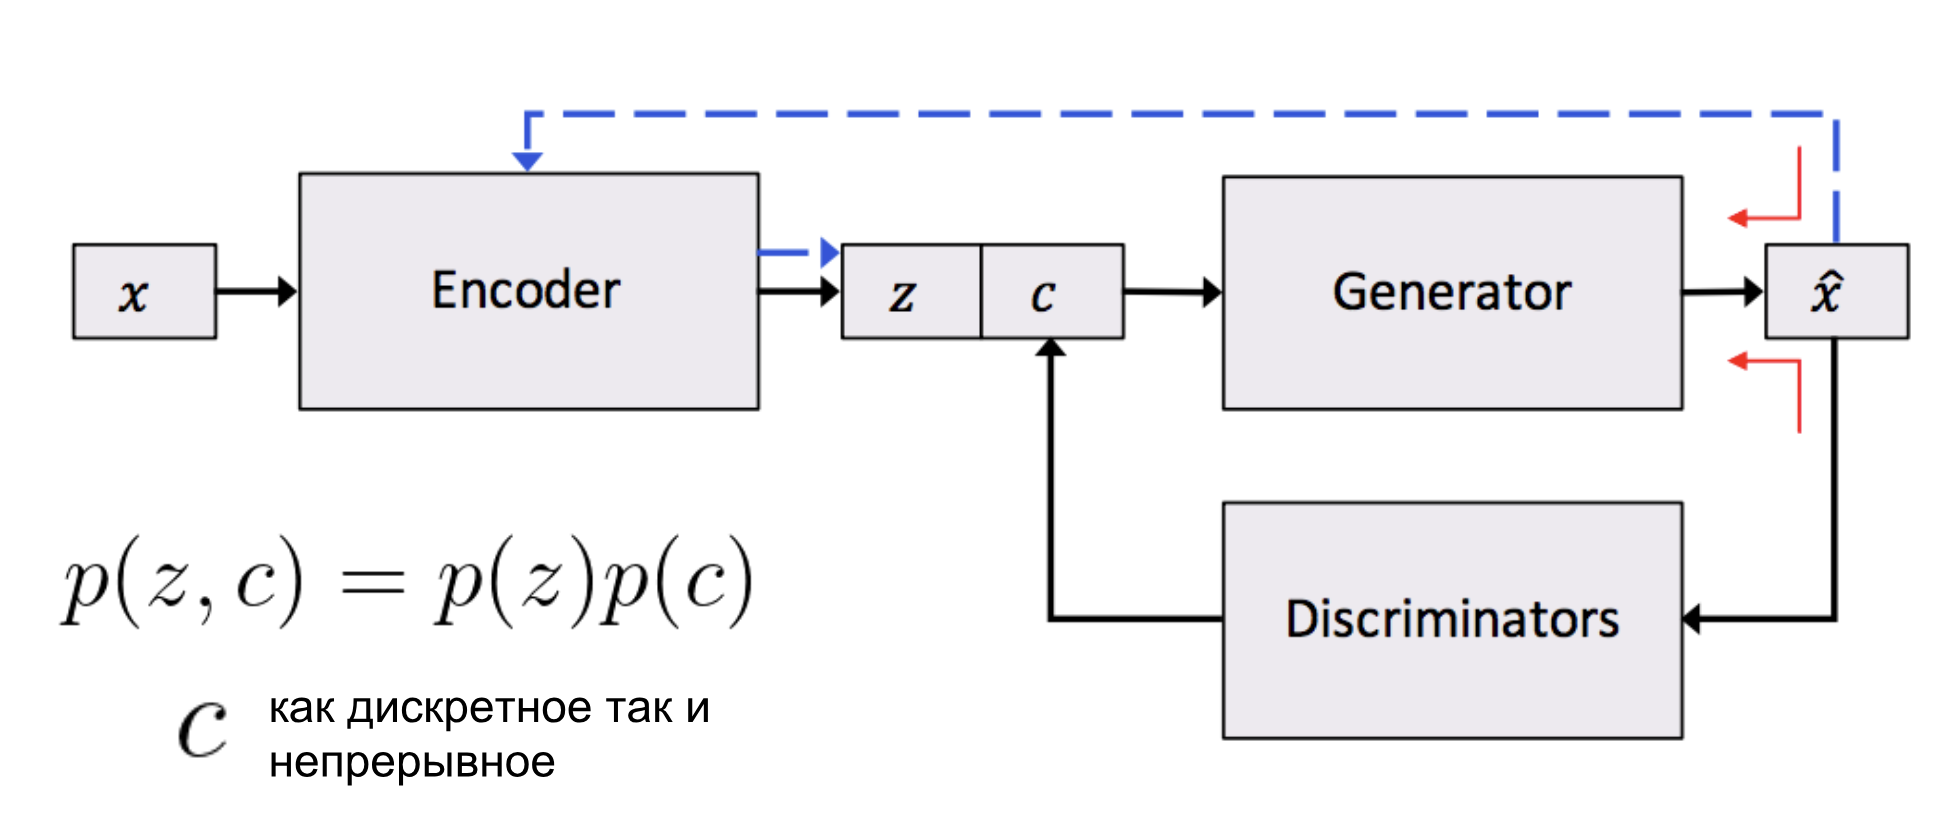
\includegraphics[width=0.7\textwidth]{images/cvae.png}
\end{center}

Реализация, основанная на CVAE (Hu et al., 2018):
\begin{itemize}
    \item В качестве дискриминатора взят CNNEncoder (Zhange et al., 2016)
    \item Вектора слов - GLoVE размерностью $100$ без заморозки
    \item WordDropout и плавное увеличение веса kl-терма по $tanh$
    \item 3-layers SRU в качестве энкодера и стохастический beam search с векторными операциями на графическом процессоре ($\sim 6x$ скорость)
    \item SGDR на Adam с $3$ рестартами для оптимизации
    \item PyTorch 0.4
\end{itemize}

\end{frame}
%-------------------------------------------------------------------------------
\begin{frame}
\frametitle{Решение}
\framesubtitle{Self-Attention}

% В данной работе удалось придумать архитектурной решение проблемы учета контекста при длинной генерации.
% это я придумал!!
% зачем - учет контекста

\begin{center}
    \begin{columns}
        \begin{column}{0.6\textwidth}
            \begin{center}
                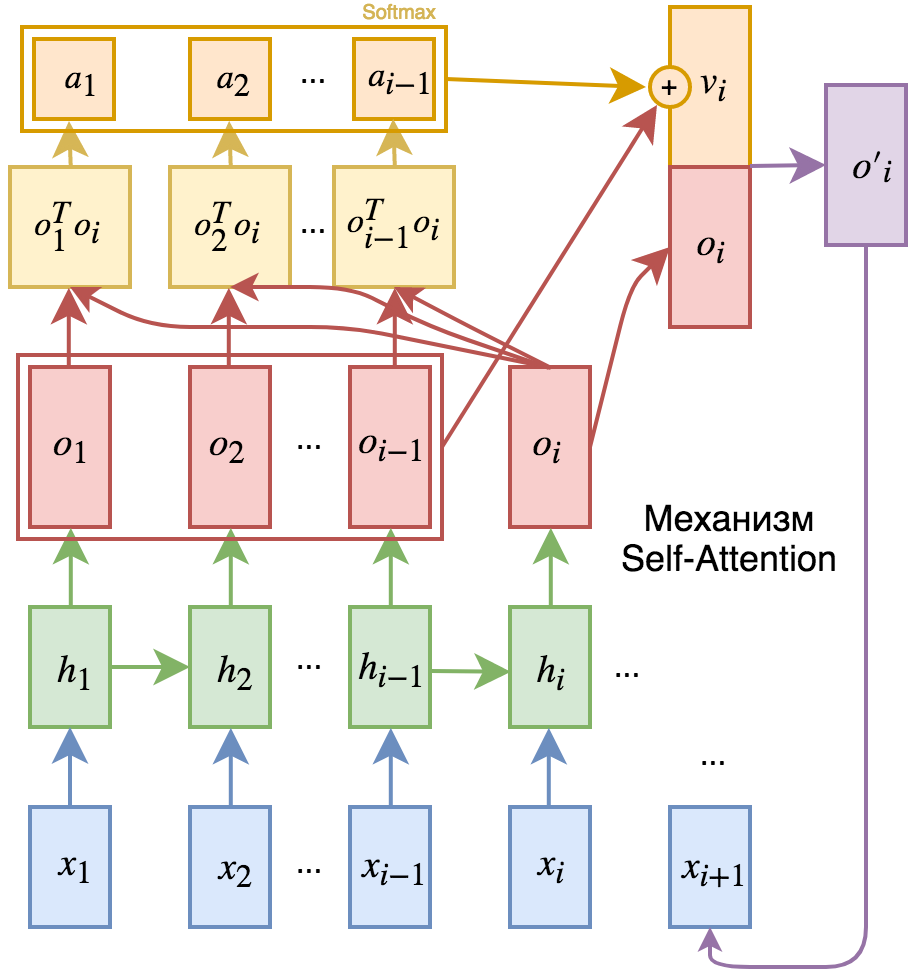
\includegraphics[width=0.95\textwidth]{images/self_attention.png}
            \end{center}
        \end{column}
        \begin{column}{0.45\textwidth}
            Расширение механизма внимания из seq2seq моделей для задач генерации:
            \begin{itemize}
                \item Используем информацию о корреляции с предыдущими представлениями на очередном шаге \textbf{декодера}.
                \item Линейный слой до и после (general), SELU активация после
                \item Зависимости можно визуализировать в виде heatmap
                \item PyTorch 0.4
            \end{itemize}
        \end{column}
    \end{columns}
\end{center}

\end{frame}
%-------------------------------------------------------------------------------
\begin{frame}
\frametitle{Решение}
\framesubtitle{Attention penalty}

% Такой штраф добавляем к логарифму совместной вероятности для учета в итоговом ранжировании. Интуитивно, чем более заполнена матрица и чем более она соответствует случаю ”каждое слово раздает единицу внимания всем другим”, тем лучше. Такой подход позволил чаще избежать вырожденных случаев при генерации (слишком коротких, повторяющихся, незаконченных), увеличив итоговые метрики.

\begin{center}
    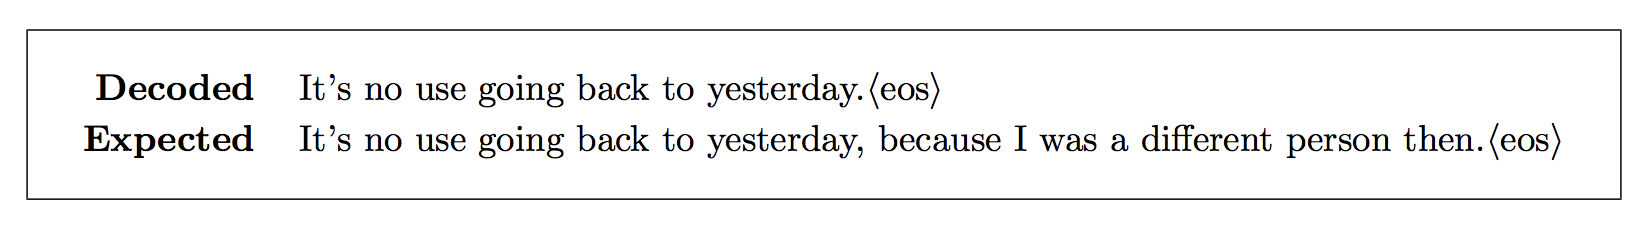
\includegraphics[width=0.8\textwidth]{images/bad_sample.png}
\end{center}

\begin{center}
    \begin{columns}[T]
        \begin{column}{0.5\textwidth}
            \begin{center}
                \vskip-5mm
                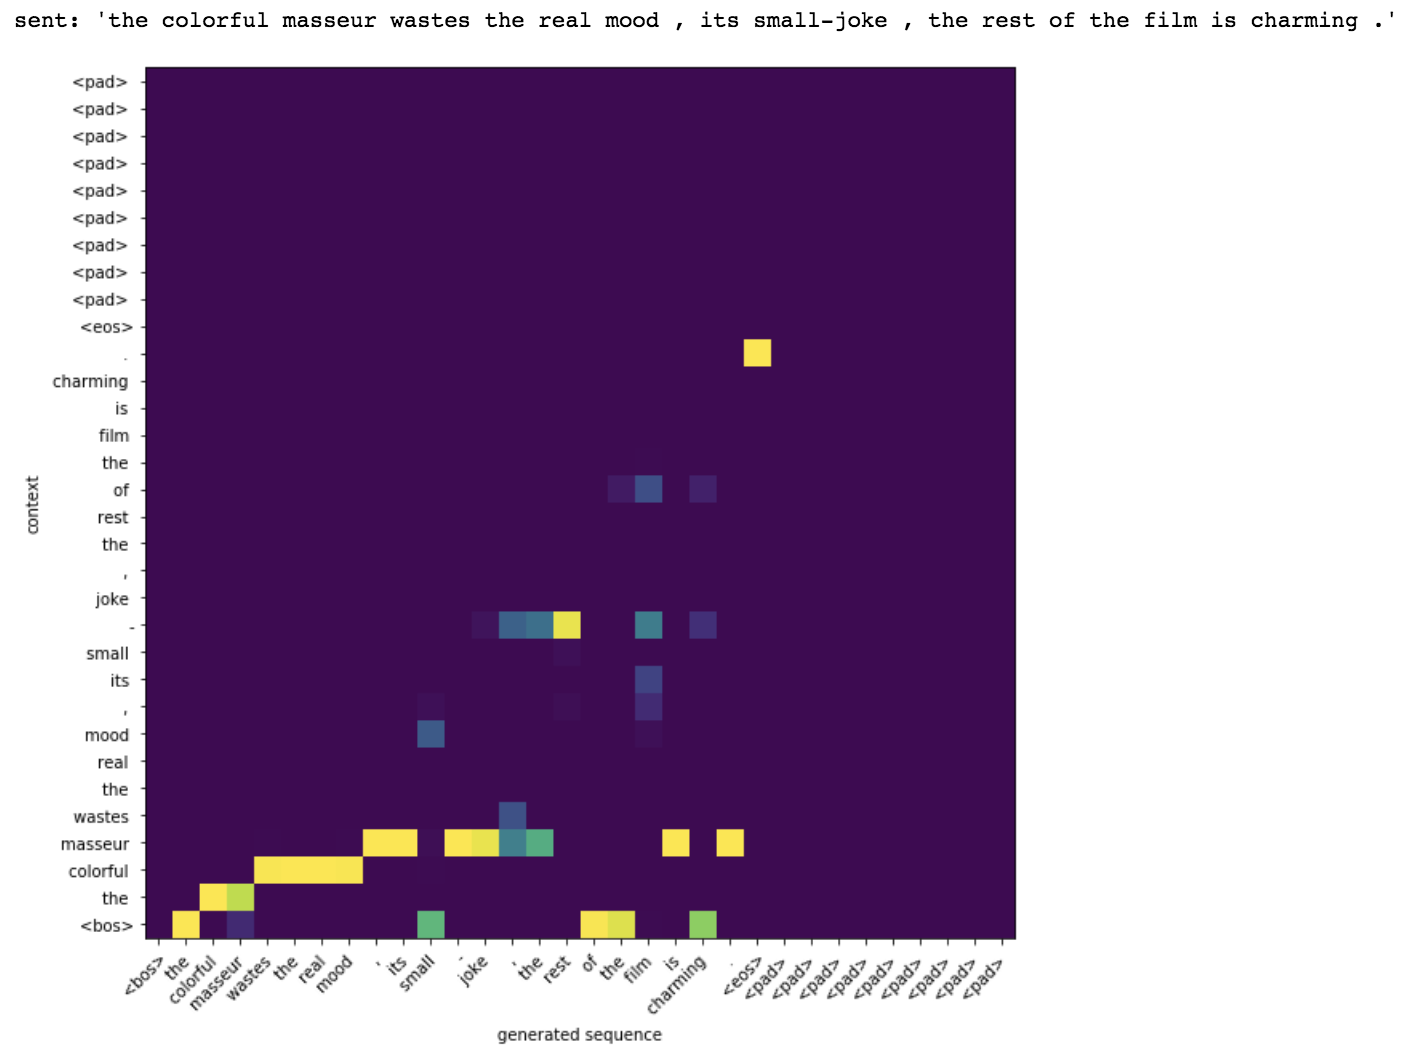
\includegraphics[width=1.4\textwidth]{images/sa_sample2.png}
            \end{center}
        \end{column}
        \begin{column}{0.5\textwidth}
            Вывод может повторяться или быть недостаточно длинным, решение:
            \begin{itemize}
                \item Каждый кандидат beam search имеет вероятность и матрицу внимания
                \item Регуляризация по весам матрицы:
                $$cp(A) = \sum\limits_{j=1}^{|x|}{\log{\left[min(\sum\limits_{i=1}^{|x|}{a_{ij}}, 1)}\right]}$$
                \item $cp(A)$ - аддитивная добавка к log-правдоподобию
            \end{itemize}
        \end{column}
    \end{columns}
\end{center}

\end{frame}
%-------------------------------------------------------------------------------
\section{Результаты}
\begin{frame}
\frametitle{Результаты}
\framesubtitle{Сравнение моделей и подходов}

% В данной главе проводится анализ результатов.
% За базовую модель, основанную на принципе максимального правдоподобия (MLE), была взять обычная рекуррентная нейронная сеть на LSTM.
% Подходы, основанные на алгоритме REINFORCE (SeqGAN, LeakGAN), сходятся крайне медленно (до нескольких дней) из-за проблем с дисперсией, а некоторые реализации не заботились о воспроизводимости вычисле- ний, поэтому использовать запустить их было проблематично. Результаты сравнения с MLE представлены на Таблице 2.
% Столь высокие показатели BLEU метрик обусловлены в том числе и тем, что в генерируемого множестве часто попадаются одинаковые или почти одинаковые сэм- плы, которые сопоставляются при подсчете n-грамм. Видно, что несмотря на высо- кие показатели BLUE, все GAN проигрывают обычному принципу максимального правдоподобия в разнообразии. Фактически, это означает, что GAN могут выдавать несколько хороших примеров, но не способны поддерживать разнообразие генерации. Одна из возможных причин - традиционная проблема с правильным сэмплировани- ем внутри алгоритма REINFORCE. Другая возможная причина связана с проблемой ”mode collapsing” [38] - главной проблемой архитектуры генеративных конкурирую- щих сетей на данный момент (Рис. 16.)
% Одно из заявленные свойств необходимого генератора - поддержание вариативно- сти, которая тут намного оказалось хуже, чем у простой базовой модели. Поэтому, модели основанные на GAN в данный момент нуждаются в решении проблемы с раз- нообразием. Похожая проблема сейчас наблюдается и в случае непрерывных данных.
% Следуя [51], точность на классификаторе DACC проверялась уже после обучения на тестовом размеченном множестве. Видно, что с заменой дискриминатора, удалось сохранить и повысить высокую точность, не ухудшив остальные метрики.
% Результаты Perplexity получились не слишком репрезентативными, оставаясь на- много позади лучших показателей в задачах языкового моделирования (это объясня- ется наличием регуляризацией на форму латентного пространства, помимо ошибки восстановления). Тем не менее, значения резко упали и при переходе к неполной раз- метки и при использовании механизма внимания, что подтверждает их полезность.
% Видно также, что резкий скачок в эффективности происходит при переходе к управляемой генерации (так мы можем использовать данные с неполной разметкой), а также при использовании механизма внимания. Стохастический beam search с ре- гуляризацией также добавляют прирост в метриках BLEU, что подтверждает их эф- фективность. При сравнении с Таблицей 2 можно наблюдать общий эффект: при увеличении правдоподобия, разнообразие по Self-BLEU тоже значительно падает, но у расширенной версии CVAE оно остается на уровне лучших GAN, сохраняя при этом высокое правдоподобие.
% Итак, предложенные оптимизации и расширения действительно смогли эффек- тивно сохранить высокую правдоподобность и относительно хорошее разнообразие, при это увеличив длину генерируемых сэмплов вдвое. При этом, мы также эффектив- но расширили модель на условия с данными с частичной разметкой (которые чаще всего можно встретить в реальной жизни), сохранив при этом высокую точность клас- сификации, а, следовательно, возможность эффективно параметризовать генератор требуемыми свойствами.

\begin{table}[H]
\begin{tabular}{c | c c c c c c}
\toprule
Metrics & SeqGAN & MaliGAN & RankGAN & LeakGAN & TextGAN & MLE \\
\midrule
BLEU & 18.0 & 15.9 & 15.6 & \textbf{23.0} & 20.7 & 8.1 \\
Self-BLEU & 48.9 & 43.7 & 61.8 & 78.0 & 74.6 & \textbf{10.6} \\
\bottomrule
\end{tabular}
\caption{BLEU5 * $100$ для $500$ сгенерированных сэмплов}
\end{table}

\begin{itemize}
    \item $D_{ACC}$ - точность классификации после генерации
    \item $CVAE_{++}$ - улучшенная реализация CVAE
    \item SA - Self-Attention, CP - штраф на матрице внимания
\end{itemize}

\begin{table}[H]
\begin{tabular}{c | c c c c}
\toprule
Metrics & VAE & CVAE & $CVAE_{++}$ + SA & \textbf{$\boldsymbol{CVAE_{++}}$ + SA + CP} \\
\midrule
$D_{ACC}$ & - & 83.483 & \textbf{84.263} & \textbf{84.263} \\
Perplexity & 150 & 104 & 84 & \textbf{83} \\
BLEU & 8.5 & 9.3 & 18.2 & \textbf{20.5} \\
Self-BLEU & 9.0 & 8.7 & 45.8 & \textbf{44.2} \\
\bottomrule
\end{tabular}
\caption{Метрики для расширений $VAE$}
\end{table}

\end{frame}
%-------------------------------------------------------------------------------
\section{Заключение}
\begin{frame}
\frametitle{Заключение}
\framesubtitle{Результаты и будущая работа}

% Современное глубокое обучение основано на способности вычислительных графов быть дифференцируемыми. При переходе к дискретным значениям старые подхо- ды перестают работать, поэтому приходиться строить отображения дискретного про- странства в непрерывное, что так или иначе ведет к проблемам с оптимизацией. За- дача генерации текста усложняется еще и тем, что при увеличении длины входных последовательностей быстро растет сложность по поддержанию связности, правдопо- добия и разнообразия генерируемых сэмплов.
% Современные генеративные модели все еще обладают рядом фундаментальных проблем, которые не позволяют считать задачу генерации решенной. Ценность этой работы заключается не только в предложенном и описанном подходе, решавшем по- ставленную задачу, но и в трудностях, возникших при реализации и тестировании, указывающих на глобальные проблемы и очерчивающих границы применимости того или иного метода или модели.

Результаты:
\begin{itemize}
    \item Изучены принципы и особенности работы генеративных моделей с дискретными значениями, намечены основные сложности, проблемы и границы применимости разных подходов.
    \item Придуманы и описаны метрики для комплексной оценки качества
    \item Придуманы и реализованы способы, позволяющие справляться с существующими проблемами и потерей качества при увеличении длины генерации (до $30$ слов).
    \item Эффективная, интерпретируемая и гибкая модель, основанная на CVAE.
\end{itemize}

Будущая работа:
\begin{itemize}
    \item Преодоление ограничения на выбор априорного и апостериорного распределения в моделях, основанных на VAE (AAE, $\alpha$-GAN).
    \item Запустить предложенную модель на дискретных не строковых данных.
\end{itemize}

\end{frame}
%-------------------------------------------------------------------------------
\section{Ссылки}
\begin{frame}
\frametitle{Ссылки}
\framesubtitle{Статьи, код и контакты}

% <silence>

\begin{center}
    {\large Спасибо за внимание!}
    \begin{enumerate}
        \item \ULurl{https://github.com/stasbel/text-gen} (Генерация)
        \item \ULurl{https://github.com/stasbel/bachelor-thesis} (Презентация)
        \item stasbelyaev96@gmail.com
        \item \ULurl{https://t.me/stasbel}
    \end{enumerate}
\end{center}

\end{frame}
%-------------------------------------------------------------------------------
%	END PRESENTATION SLIDES
%-------------------------------------------------------------------------------
\end{document}